\documentclass[11pt,spanish,a4paper]{article}
% Versión 1.er cuat 2021 Víctor Bettachini < bettachini@df.uba.ar >

% Versión 1.er cuat 2021 Víctor Bettachini < bettachini@df.uba.ar >

\usepackage[T1]{fontenc}
\usepackage[utf8]{inputenc}

\usepackage[spanish, es-tabla]{babel}
\def\spanishoptions{argentina} % Was macht dass?
% \usepackage{babelbib}
% \selectbiblanguage{spanish}
% \addto\shorthandsspanish{\spanishdeactivate{~<>}}

\usepackage{graphicx}
\graphicspath{{./figuras/}{../LaTeX/}}
% \usepackage{float}

\usepackage[arrowdel]{physics}
\newcommand{\pvec}[1]{\vec{#1}\mkern2mu\vphantom{#1}}
% \usepackage{units}
\usepackage[separate-uncertainty=true, multi-part-units=single, locale=FR]{siunitx}
\usepackage{isotope} % $\isotope[A][Z]{X}\to\isotope[A-4][Z-2]{Y}+\isotope[4][2]{\alpha}

\usepackage{tasks}
\usepackage[inline]{enumitem}
% \usepackage{enumerate}

\usepackage{hyperref}

% \usepackage{amsmath}
% \usepackage{amstext}
\usepackage{amssymb}

\usepackage{tikz}
\usepackage{tikz-dimline}
\usetikzlibrary{calc}
% \usetikzlibrary{math}
\usetikzlibrary{arrows.meta}
\usetikzlibrary{snakes}
\usetikzlibrary{decorations}
\usetikzlibrary{decorations.pathmorphing}
\usetikzlibrary{patterns}

% \usepackage[hmargin=1cm, vmargin=1cm, includeheadfoot]{geometry}
\usepackage[hmargin=1cm,vmargin=3cm, top= 0.75cm,nohead]{geometry}
% \voffset-3.5cm
% \hoffset-3cm
% \setlength{\textwidth}{17.5cm}
% \setlength{\textheight}{27cm}

\usepackage{lastpage}
\usepackage{fancyhdr}
\pagestyle{fancyplain}
\fancyhf{}
% \fancyhead{}
\setlength\headheight{28.7pt} 
\fancyhead[LE, LO]{\textbf{Física 2} (Físicos) }
% \lhead{\textbf{Física 2} (Físicos) }
\fancyhead[RE, RO]{\href{https://df.uba.ar/es/}{$\vcenter{\hbox{\includegraphics[height=1cm]{sin_texto.pdf}}}$}}
% \rhead{$\vcenter{\hbox{\includegraphics[height=1cm]{sin_texto.jpg}}}$}
% \rhead{\includegraphics[height=1cm]{sin_texto.jpg}}
% \rhead{\textcopyright {\tt DF, FCEyN, UBA}}
\fancyfoot{\href{https://creativecommons.org/licenses/by-sa/4.0/deed.es/}{$\vcenter{\hbox{\includegraphics[height=0.4cm]{cc-by-sa.pdf}}}$} \href{https://df.uba.ar/es/}{DF, FCEyN, UBA}}
% \fancyfoot{$\vcenter{\hbox{\includegraphics[height=0.4cm]{cc-by-sa.pdf}}}$ DF, FCEyN, UBA}
% \fancyfoot{{\tiny \textcopyright DF, FCEyN, UBA}}
\fancyfoot[C]{ {\tiny Actualizado al \today} }
\fancyfoot[RO, LE]{Pág. \thepage/\pageref{LastPage}}
\renewcommand{\headrulewidth}{0pt}
\renewcommand{\footrulewidth}{0pt}


\begin{document}
\begin{center}
	\textbf{Física 2} (Físicos) \hfill \textcopyright {\tt DF, FCEyN, UBA}\\
	\textsc{\LARGE N\textgreater\textgreater1 grados de libertad forzados}
\end{center}

Los ejercicios con (*) entrañan una dificultad adicional. Son para investigar después de resolver los demás.


\begin{enumerate}

				
\item
\begin{minipage}[t][3.5cm]{0.6\textwidth}
Este arreglo lineal de péndulos acoplados tiene extremos en $z= 0$ y en $z= L$.
Se aplica una fuerza externa en función del tiempo a la primera masa ($z=0$), de forma tal que se conoce su amplitud $\Psi(0,t)= A_0 \cos(\Omega t)$.
Halle el movimiento estacionario del sistema y discuta las hipótesis que hace.
Compare con el caso de extremo derecho fijo a una pared (o sea: agregando un resorte a la derecha de la última masa y uniéndolo a la pared). 
\end{minipage}
\begin{minipage}[c][0cm][t]{0.35\textwidth}
  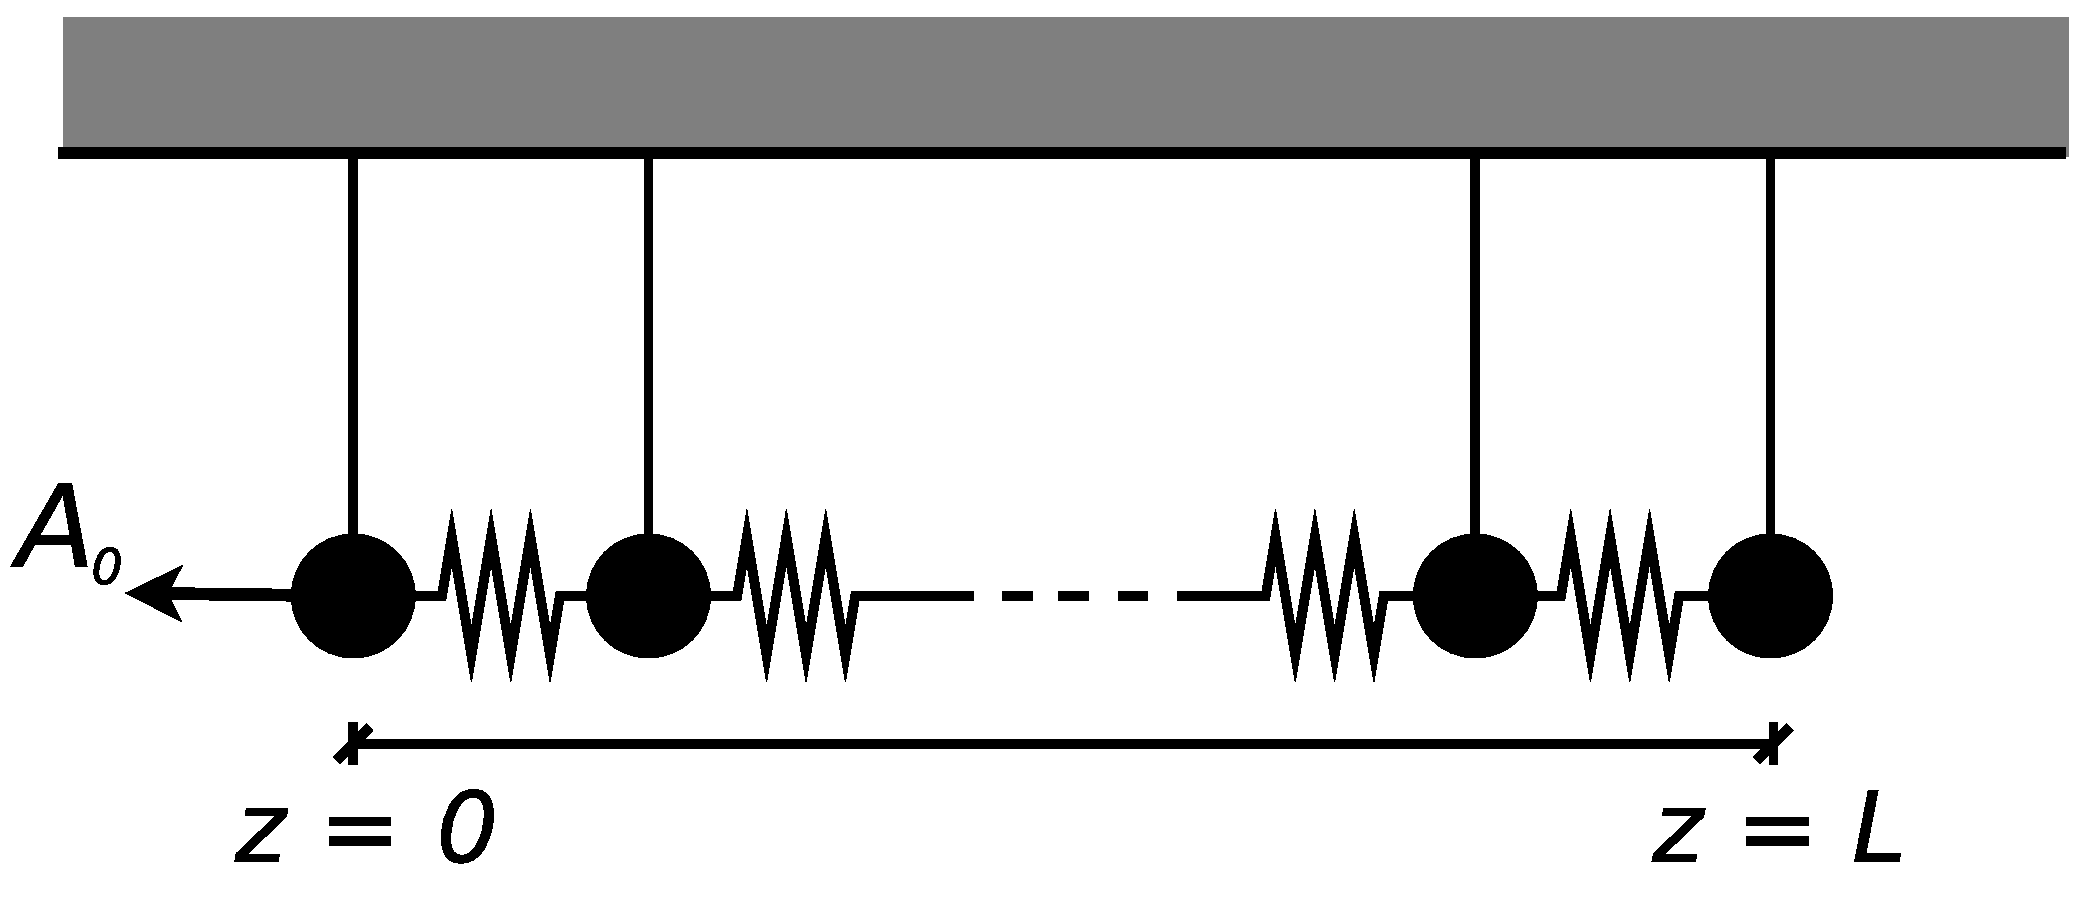
\includegraphics[width=\textwidth]{ej1-15}
\end{minipage}



\item
\begin{minipage}[t][3cm]{0.35\textwidth}
Considere un sistema de péndulos acoplados con un cambio brusco en $\omega_{0}^{2}$ en $z=L$, según se esquematiza en la figura.
\end{minipage}
\begin{minipage}[c][3cm][t]{0.6\textwidth}
  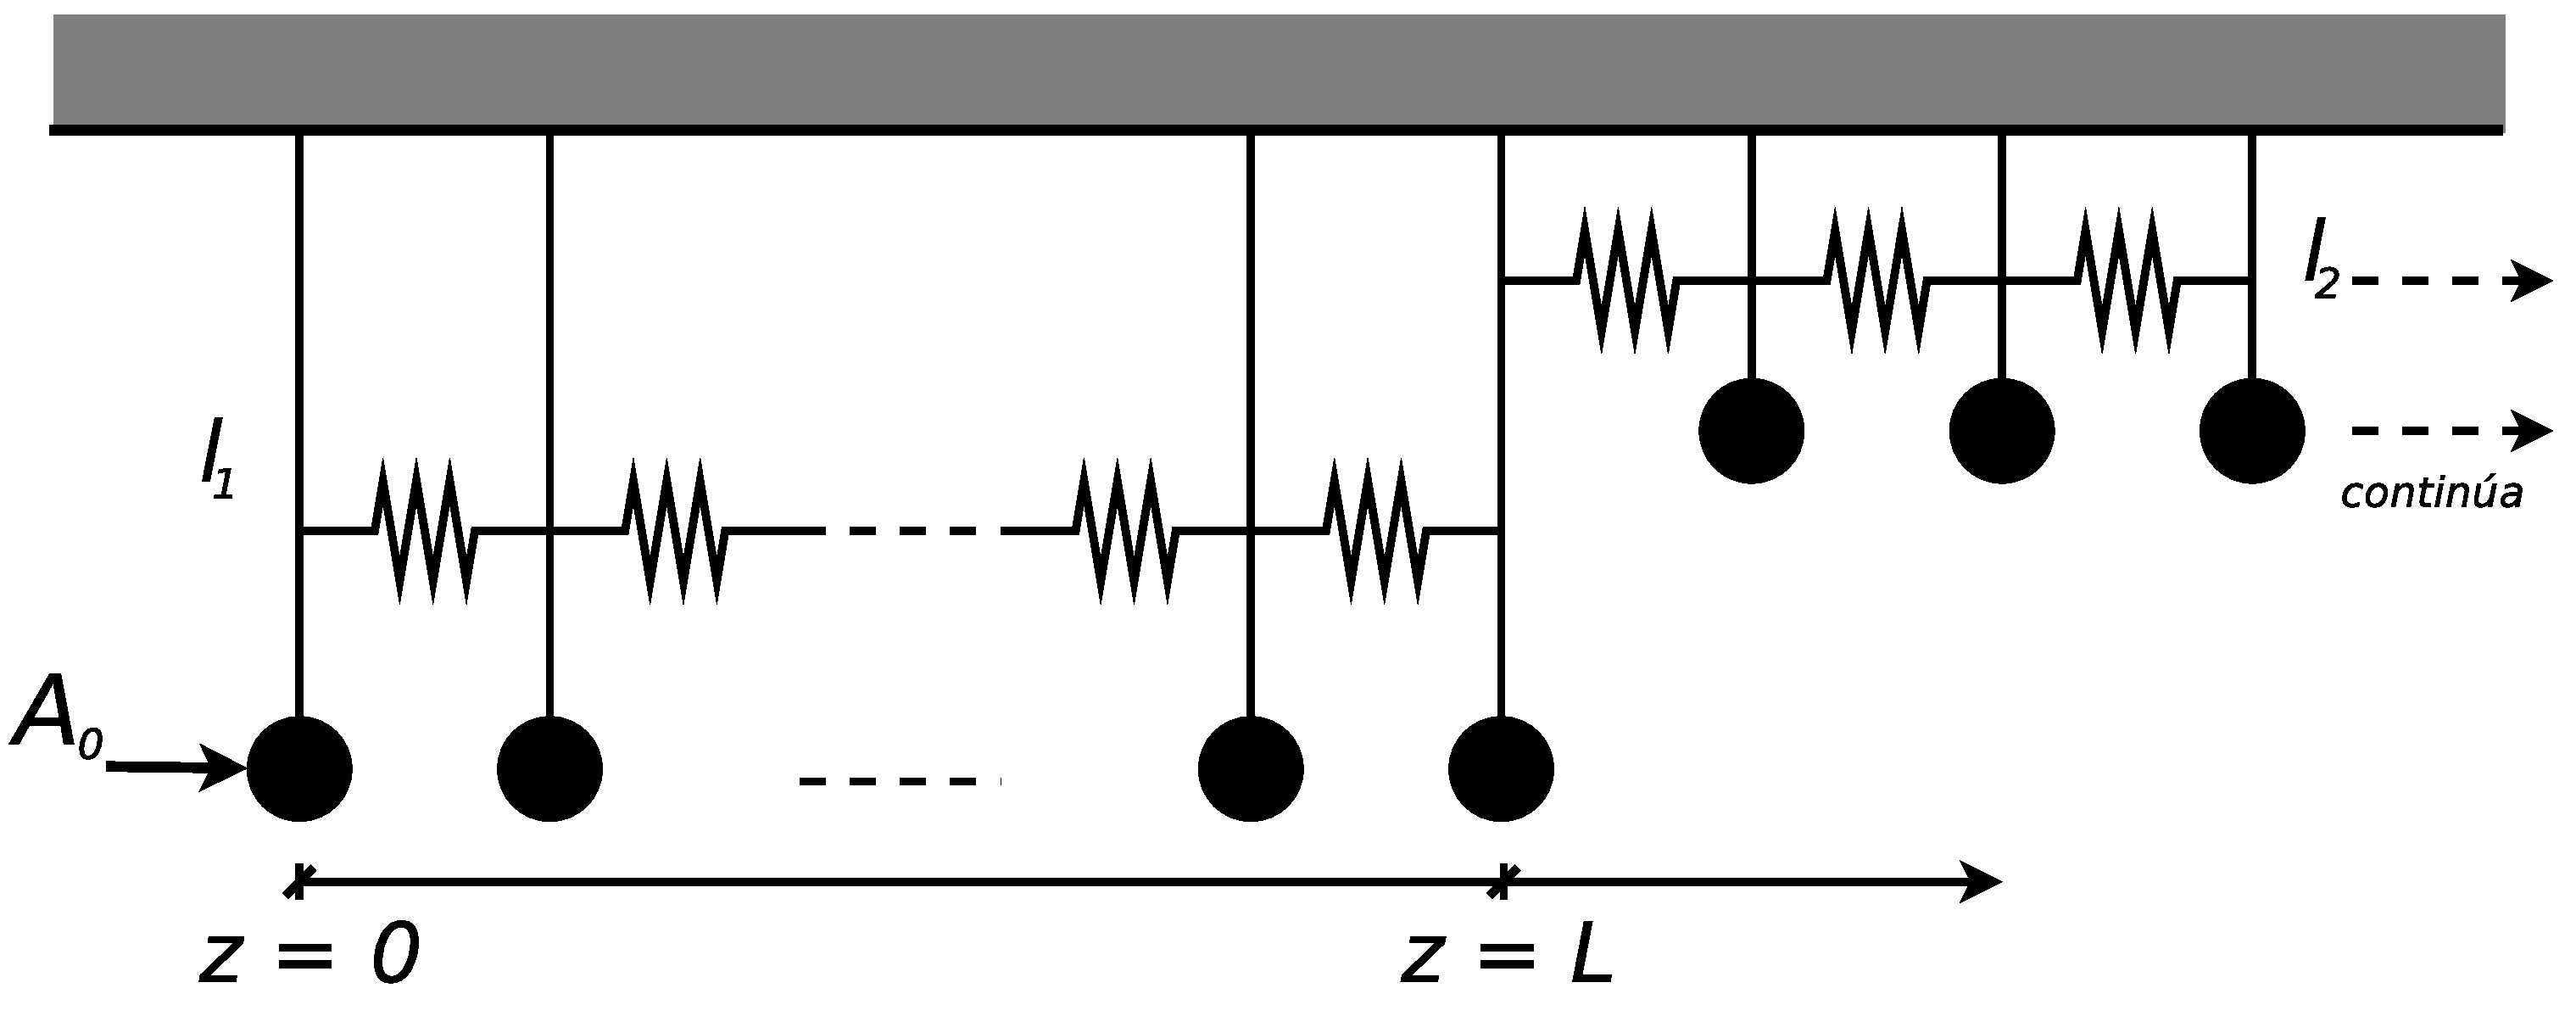
\includegraphics[width=\textwidth]{ej1-16}
\end{minipage}
\begin{enumerate}
	\item Discuta cómo tiene que ser \(\Omega\) para que el sistema se comporte como dispersivo en \(0< z < L\) y reactivo en \(z > L\).
	¿Cuál sería la relación entre \(l_1\) y\(l_2\)?
	\item En dichas condiciones estudie el movimiento estacionario del sistema y encuentre las frecuenciasde resonancia.
	\item ¿Qué pasa ahora si se invierte la relación entre \(l_1\) y \(l_2\)?
	¿De qué variable depende el comportamiento en \(z > L\)?
	\item ¿Es posible encontrar un rango de frecuencias \(\Omega\) tal que el sistema se encuentre en el mismo rango de comportamiento en \(0< z < L\) y en \(z > L\)?
\end{enumerate}



\item
\begin{minipage}[t][3.5cm]{0.45\textwidth}
Para el sistema esquematizado en la figura, calcule $\Psi_{n}(t)$, si $\Omega<\omega_\textrm{mín}$.
\end{minipage}
\begin{minipage}[c][2cm][t]{0.5\textwidth}
  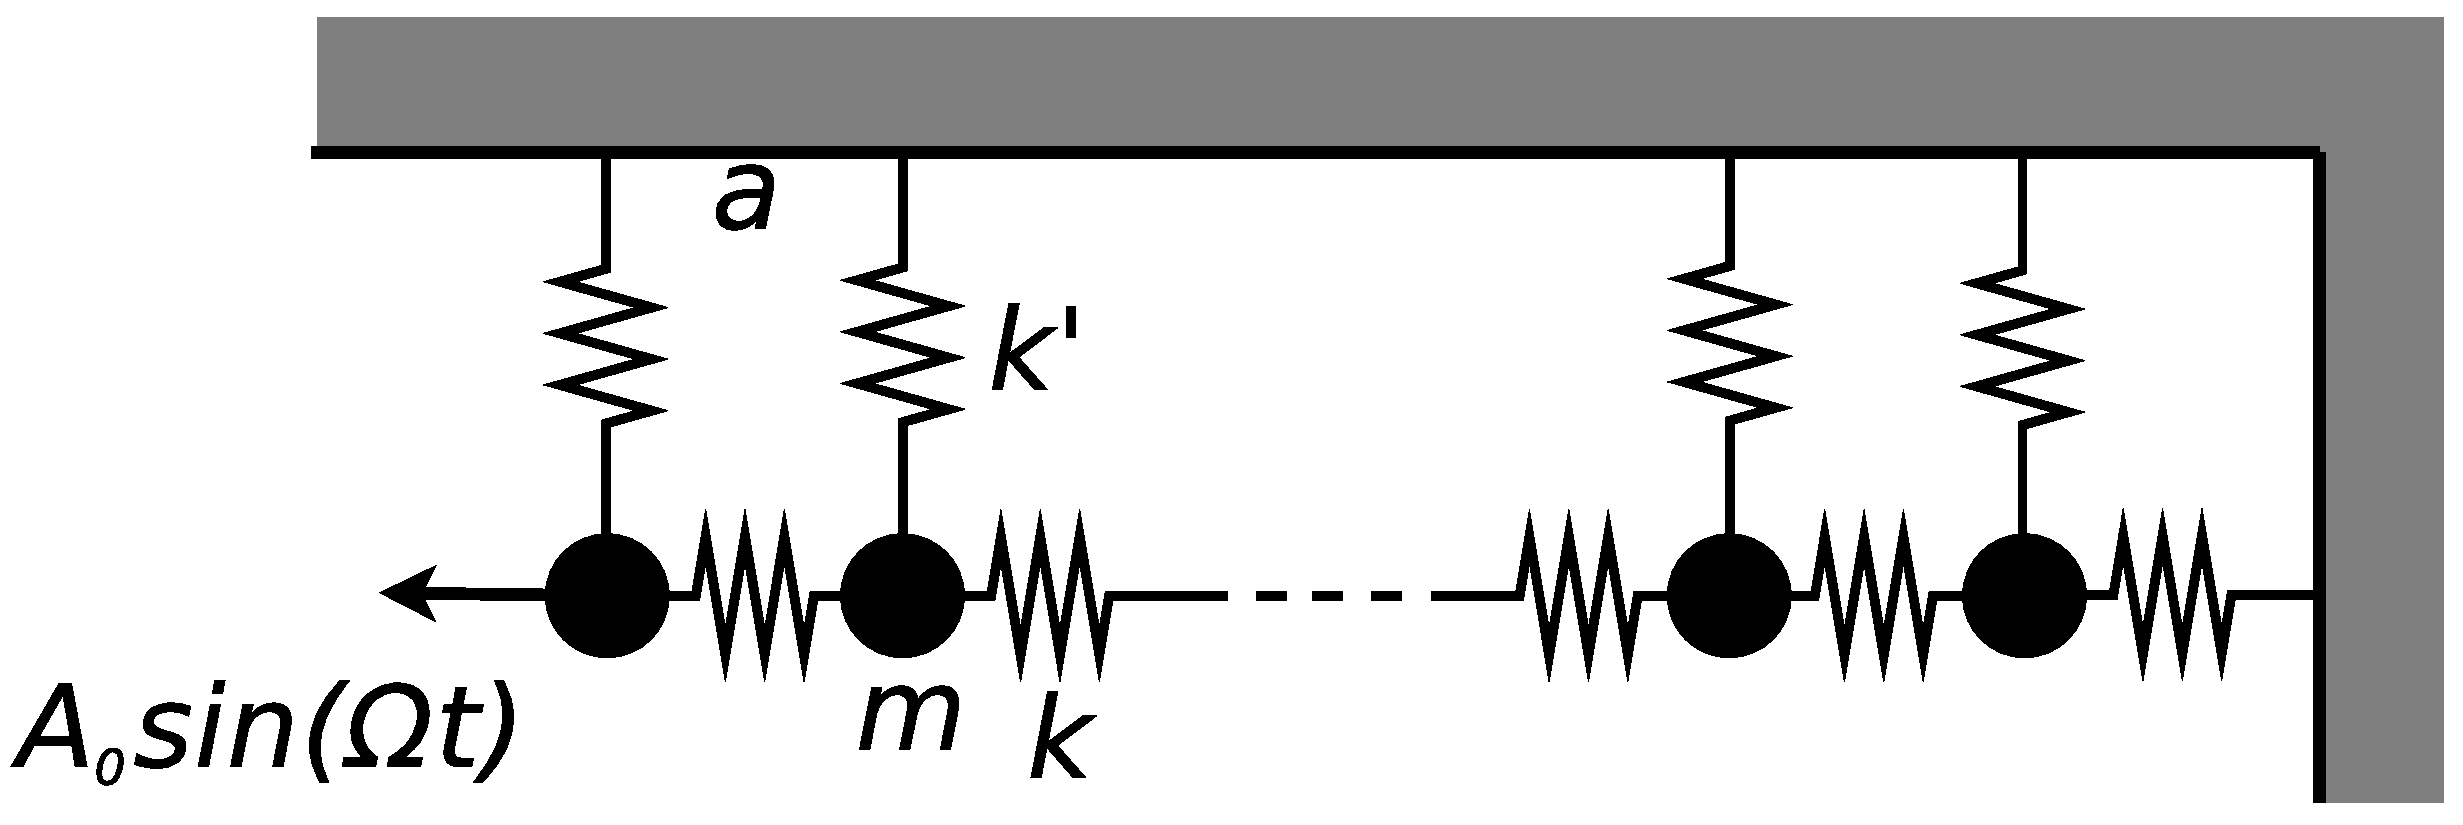
\includegraphics[width=\textwidth]{ej1-17}
\end{minipage}




\end{enumerate}

\end{document}
